%% Aggregate Accuracy Does Not Reveal Reliability -- ISPRS Journal of Photogrammetry and Remote Sensing (Elsevier)
%% Compile on Overleaf (has elsarticle + natbib) or locally with: latexmk -pdf main.tex
%% Figures fig2_flagship_reliability.pdf and fig3_domain_gaps.pdf must be in the same directory.
\documentclass[preprint,3p,times]{elsarticle}

\usepackage{amsmath,amssymb}
\usepackage{graphicx}
\usepackage{booktabs}
\usepackage[hidelinks]{hyperref}
\usepackage{textcomp}
\setlength{\emergencystretch}{2em}   % absorb the few minor overfull lines gracefully

\journal{ISPRS Journal of Photogrammetry and Remote Sensing}

\begin{document}

\begin{frontmatter}

\title{Aggregate Accuracy Does Not Reveal Reliability: Silent Conformal Certificate Failure under Operational Spectral and Domain Shift in Sentinel-2 Cloud Segmentation}

\author[a]{Hsiu-Chi Tsai\corref{cor1}}
\ead{hctsai1006@cs.nctu.edu.tw}
\author[b]{Chia-Tung Chung}
\ead{jun.514114.ee10@nycu.edu.tw}
\cortext[cor1]{Corresponding author.}
\affiliation[a]{organization={Arete Honors Program, National Yang Ming Chiao Tung University}, city={Hsinchu}, country={Taiwan}}
\affiliation[b]{organization={Department of Photonics, National Yang Ming Chiao Tung University}, city={Hsinchu}, country={Taiwan}}

\begin{abstract}
Operational Earth observation increasingly relies on deep segmentation models whose outputs gate downstream pipelines, and a large literature measures how well they retain their \emph{accuracy} under operational distribution shift---atmospheric correction, sensor changes, unseen geographies and surfaces. We show that accuracy-robustness is not enough: a conformal certificate calibrated before deployment and reused under shift without revalidation can be actively misleading, failing by far more than an aggregate accuracy drop would signal while that drop itself hides a per-class collapse. Using split conformal risk control on real Sentinel-2 cloud segmentation (CloudSEN12), we demonstrate that under the operational L1C$\to$L2A atmospheric-correction shift a model's \emph{reliability degrades disproportionately to its accuracy, and silently}: pixel accuracy falls 12 points ($79.5 \to 67.1\,\%$) while a clean-calibrated conformal threshold's confidently-wrong (joint) risk rises more than threefold, from $8.5\,\%$ to $28.9 \pm 0.5\,\%$ against a $10\,\%$ target---a $+20$-point rise the calibration statistic it minimises never reports, because that statistic stays below target by construction. Per-stratum (Mondrian) recalibration restores the joint-risk target ($8.6 \pm 0.2\,\%$; paired gap $+20.3 \pm 0.5$, two-way cluster-robust standard error over 100 runs), but by abstaining: coverage falls from $93$ to $45\,\%$ and the error \emph{among accepted} pixels remains $19.4\,\%$---both of which we report rather than hide. The failure is not an artefact of one processor, one scene set, or one operating point: a second, algorithmically different atmospheric processor (ACOLITE) breaks the same certificate to a statistically equivalent degree ($28.6\,\%$, paired difference within a $\pm2\,\%$ margin), the breach replicates on the official held-out validation scenes ($29.1\,\%$, audited for shared train products), and it persists across target risks from $5$ to $20\,\%$; nor does a covariate-shift-aware weighted-conformal threshold---a likelihood-ratio approximation or a confidence-density heuristic---repair it, because the shift moves the confidence-to-error relationship, not merely the covariate density that reweighting corrects. We trace the breach to a stale input-normalization contract---the model normalizes L2A with its L1C training statistics---and find that re-normalizing each product with its own unlabelled statistics restores the joint risk to $10.2\,\%$ at $74\,\%$ coverage: a label-free repair at clean-like coverage, without the target labels or the abstention that the per-stratum recalibration above requires. We then show the failure is conditional rather than universal. Among pure deployment shifts (input held fixed), a structural surface gap (deploying on unseen bright surfaces) pushes the naive risk above target ($11.4 \pm 0.3\,\%$, significant under the two-way SE but not under a scene-resampling bootstrap; restored to $2.4\,\%$), while a milder geographic gap (train Northern hemisphere, deploy Southern) does not ($9.8\,\%$, its interval including the target). The reliability crisis is therefore \emph{conditional} on the kind of shift---an illustrative contrast between two deployment shifts, not a general diagnosis or a necessary-condition law. It is also model-dependent: a channel-adaptive foundation model (DOFA), run through the \emph{identical} protocol, is far more reliable under the atmospheric shift (naive joint risk $9.9\,\%$ versus $28.9\,\%$ for the small model, sitting at the target rather than far above it), though it is not immune---a spectral-band-drop shift raises its naive risk to a modest, certified breach. Isolating spatial context in one harness, a from-scratch spatial U-Net breaches too but far less than a per-pixel model on identical nine-band data ($13.1$ versus $24.2\,\%$), and the label-free re-normalization restores both; the severity is thus progressively attenuated by spatial context and pretraining, not a per-pixel artefact. Throughout, we report every risk with its coverage, because the certified quantity is a joint mass that abstention alone can drive to zero. Methodologically, a defensible certificate on this data requires a scene-connected-component exchangeable unit (Sentinel-2 products that span multiple annotation regions violate ROI-level exchangeability) and a two-way cluster-robust standard error over the crossed calibration-split $\times$ model-seed design. To our knowledge this is the first study to measure conformal-certificate \emph{failure} for Sentinel-2 optical segmentation under a real atmospheric-correction shift, with a scene-level exchangeable unit and an initial characterisation of when it occurs; conformal and selective prediction have concurrently been taken to other operational remote-sensing shifts, but not to this one.
\end{abstract}

\begin{keyword}
conformal prediction \sep uncertainty quantification \sep distribution shift \sep cloud segmentation \sep Sentinel-2 \sep operational reliability
\end{keyword}

\end{frontmatter}

\section{Introduction}
Earth-observation segmentation models are moving from research benchmarks into operational pipelines: cloud masking that gates every downstream surface-reflectance product, land-cover mapping that feeds policy, change detection that triggers alerts. In these settings the model rarely sees the exact distribution it was trained on. The Sentinel-2 archive alone exposes a model to at least four operational shifts: the L1C$\to$L2A atmospheric correction that transforms top-of-atmosphere reflectance to bottom-of-atmosphere reflectance and removes the cirrus band B10; cross-sensor transfer as constellations evolve; deployment across geographies and seasons absent from the training set; and deployment on surface types (bright built-up, bare soil, snow and ice) that are both operationally critical for cloud confusion and under-represented in labelled data.

A substantial literature now measures how well models \emph{maintain accuracy} under such shifts. Channel- and sensor-adaptive encoders \citep{xiong2024dofa,waldmann2025panopticon,francis2021sensei,bao2024channelvit} are evaluated on their cross-band and cross-sensor accuracy; robustness benchmarks score accuracy under image-space corruptions \citep{li2025reobench}; cross-band generalisation studies quantify accuracy transfer across spectral-band configurations \citep{tamazyan2025geocrossbench}. What this literature does not ask is whether, \emph{under the same shifts}, the model still \textbf{knows when it is wrong}---whether the uncertainty it reports remains trustworthy. That question is not a refinement of accuracy-robustness; the two can decouple. A model can preserve its mean accuracy while its confidence-to-error relationship silently drifts, so that a fixed operating point calibrated before deployment admits far more confident errors than it certifies.

Conformal prediction offers a principled way to \emph{certify} such an operating point: split conformal and its risk-controlling variants give a finite-sample guarantee on a chosen error notion. But the guarantee holds only under exchangeability between calibration and test data, and operational shift is precisely a controlled violation of exchangeability. The danger is not that the certificate fails loudly---it is that it fails \emph{silently}: the calibration-set statistic the procedure minimises stays below target by construction, so a practitioner reading only that number sees success, while the deployed risk runs above target with nothing to announce it.

This paper makes that failure concrete, operational, and---crucially---bounded. Our contributions are:
\begin{itemize}
\item \textbf{C1 --- Reliability degrades disproportionately to accuracy, and silently, under a real atmospheric shift.} On CloudSEN12, under the genuine L1C$\to$L2A Sen2Cor transition (not a synthetic ablation), pixel accuracy falls 12 points while a clean-calibrated conformal threshold's confidently-wrong joint risk more than triples to $28.9\,\%$ against a $10\,\%$ target. The reliability breach is disproportionate to the accuracy loss and is never announced, since the certificate's own calibration statistic still passes (Section~\ref{sec:flagship}).
\item \textbf{C2 --- Whether the failure occurs is conditional on the kind of shift, and its severity is model-dependent.} Two pure deployment shifts (input held fixed) separate the conditions: a structural surface gap raises the naive risk above target ($11.4\,\%$, significant under the two-way SE but scene-composition-sensitive), while a milder geographic gap gives no clear evidence of a breach ($9.8\,\%$, close to target). Together these are an illustrative contrast between two deployment shifts, not a general diagnosis and not a claim that severity tracks a measured gap size. The severity is also model-dependent: isolated in one harness, spatial context attenuates the breach (a per-pixel model $24.2\,\%$, a spatial U-Net $13.1\,\%$ on identical nine-band data) and pretraining attenuates it further (DOFA $9.9\,\%$), so the crisis is progressively softened by model class rather than universal (Sections~\ref{sec:deployment}--\ref{sec:modelclass}).
\item \textbf{C3 --- The mechanism is a stale normalization contract, and the first remedy needs no labels.} We trace the atmospheric breach to a stale input-normalization contract---the model normalizes each product with its source (L1C) training statistics and reuses them on L2A---and show that re-normalizing the deployment product with its \emph{own} unlabelled statistics restores the certificate at clean-like coverage, without target labels or abstention (Section~\ref{sec:flagship}). Where a residual remains or the shift is not a normalization change (the surface gap), per-stratum (Mondrian) recalibration on target-state labels is a second, costlier remedy; because the certified quantity is a joint mass that abstention alone can drive to zero, we report every risk with its coverage and quantify the coverage each remedy spends.
\item \textbf{C4 --- The methodology a defensible certificate on this data requires.} The exchangeable unit must be the scene-connected component, not the annotation ROI---12 Sentinel-2 products in the CloudSEN12 test split each appear under two ROIs, so ROI-level splitting leaks a scene across calibration and test---and the standard error over the crossed calibration-split $\times$ model-seed design must be two-way cluster-robust rather than treating the 100 cells as independent (Section~\ref{sec:method}).
\end{itemize}

We are deliberate about scope. We claim only the \emph{operational instantiation}: that a naive conformal certificate can lose its validity under distribution shift is established theory (the coverage-gap bound of \citet{barber2023}, and the online treatment of \citet{gibbs2021}), with weighted conformal a known remedy under known covariate shift \citep{tibshirani2019}; the risk-control machinery is borrowed \citep{angelopoulos2024}; per-stratum recalibration is a Mondrian special case \citep{vovk2005}; and the label-free repair we find is a known test-time-normalization remedy \citep{schneider2020,tent2021,dua2022,corley2024}, applied here to the input rather than to internal batch statistics. Our mechanism components (band-group tokenisation, wavelength-conditioned attention, spectral-group masked pretraining, band-group dropout) are cited reused ingredients, not claimed contributions. What is new is the demonstration, diagnosis and honest costing of this \emph{silent} certificate failure for operational remote-sensing segmentation on real Sentinel-2---that a routine calibration-to-deployment product-normalization mismatch silently invalidates the certificate while its own statistic still passes, and that a label-free product-aware re-normalization repairs it---together with the exchangeability and variance methodology that makes the demonstration defensible.

\section{Related work}
\paragraph{Conformal prediction under distribution shift.} Split conformal prediction gives distribution-free finite-sample coverage under exchangeability; when calibration and test distributions differ, coverage is no longer guaranteed. Weighted conformal prediction \citep{tibshirani2019} recovers validity under \emph{known} covariate shift; \citet{barber2023} bound the coverage gap under general non-exchangeability; \citet{gibbs2021} and \citet{podkopaev2021} treat online and label shift, and \citet{cauchois2024} give distributionally-robust coverage over a bounded shift set. Conformal risk control \citep{angelopoulos2024} generalises coverage to monotone risks and is the machinery we adopt. Where coverage deviation under shift has been examined in a hyperspectral Raman-imaging setting it has been treated as an \emph{observable}, label-dependent diagnostic \citep{booksh2025}---the opposite of the silent failure we characterise here, in which the certificate's own statistic never signals the breach. We use none of these to \emph{fix} the shift---our naive arm is deliberately an unweighted certificate, so that its failure is the measurement; the remedy we study is the simplest valid instance, per-stratum (Mondrian, \citealt{vovk2005}) recalibration on discrete operational states.

\paragraph{Conformal and selective prediction in remote sensing.} Conformal methods have reached remote sensing, most often \emph{in distribution}: split-conformal hyperspectral classification with a within-scene permutation-invariance assumption to repair exchangeability \citep[SACP,][]{liu2024sacp}, and conformal \emph{risk} control for semantic segmentation---including the LoveDA aerial benchmark---with image-level exchangeability and no deployment shift \citep{mossina2024}. A smaller, largely concurrent line takes conformal or selective prediction to \emph{operational} shifts: out-of-calibration detection on scene classification under simulated corruption \citep{bhattacharjee2024}, spatial-covariate-shift conformal regression for satellite-derived air quality that measures coverage collapse \citep{adjei2026}, and out-of-distribution-triggered selective abstention in Earth-observation foundation models \citep{shrugfm2025}, and conformal prediction for Sentinel-2 flood segmentation \citep{floodconformal2025}. Our work differs from all of these in the three respects that define an operational reliability claim: it measures what happens to the conformal \emph{certificate itself} under a real atmospheric-correction (L1C$\to$L2A) shift on optical Sentinel-2 segmentation, rather than assuming exchangeability or testing a synthetic corruption; it makes the \emph{scene-connected component} the exchangeable unit, because pixel- and image-level exchangeability are broken by intra-scene correlation and by the shift; and its contribution is the \emph{measurement of certificate failure}---the robustness $\neq$ reliability decoupling---not the in-distribution production of prediction sets.

\paragraph{Robustness $\neq$ reliability.} The decoupling of accuracy-robustness from uncertainty-reliability has been observed outside remote sensing---under natural and medical distribution shift, chiefly through calibration and expected-calibration-error rather than conformal risk \citep{roschewitz2025,ovadia2019}. We give what is, to our knowledge, the first measurement of this decoupling for a conformal \emph{certificate} under a real atmospheric-correction shift in remote sensing.

\paragraph{Channel-adaptive and missing-band remote sensing.} Sensor- and channel-adaptive encoders \citep{xiong2024dofa,waldmann2025panopticon,francis2021sensei} and channel-sampling regularisers \citep{bao2024channelvit,pham2024dichavit} target \emph{accuracy} under varying or missing bands. We engage this literature as the source of our (cited) mechanism components and, in a companion decomposition (summarised in Section~\ref{sec:disc} and released with the code), by showing which ingredients actually carry missing-band robustness and how that carrying is itself regime-dependent.

\section{Method}
\label{sec:method}
\subsection{Task, data, and models}
We study per-pixel cloud segmentation on CloudSEN12 \citep{aybar2022cloudsen12}, a Sentinel-2 benchmark of expert-labelled cloud and cloud-shadow masks with co-registered L1C (top-of-atmosphere, 13 bands) and L2A (Sen2Cor bottom-of-atmosphere, 12 bands; B10 removed, \citealt{mainknorn2017sen2cor}) products for the identical pixels. We deliberately study per-pixel spectral segmentation without spatial context, so that the reliability signal we measure is spectral and not a function of spatial redundancy; a spatial-context foundation-model baseline is included in Section~\ref{sec:modelclass}. The classes are clear, thick cloud, thin cloud, and cloud shadow. We use the manually-annotated \emph{high}-quality tier of the original CloudSEN12 release (as opposed to its scribble and unlabelled tiers), which already provides the paired L1C/L2A products our design needs, with the exact scene manifest in the released code; a re-run on the extended CloudSEN12+ labels is a label-version sensitivity check we leave to future work.

Our primary model is a band-as-modality encoder: physically-grouped spectral bands are tokenised, given a wavelength-conditioned positional encoding, mixed by cross-band attention, and pretrained with a spectral-group masked autoencoder before supervised fine-tuning with band-group dropout. This architecture is not a contribution---every ingredient is a cited reused component---but a substrate on which to measure reliability; we include a plain multilayer-perceptron baseline (with and without band-group dropout) and, in Section~\ref{sec:modelclass}, a frozen channel-adaptive foundation model \citep[DOFA,][]{xiong2024dofa}.

\subsection{Reliability framework}
For a fixed trained model we score every test pixel $p$ by its maximum softmax probability $c_p$ after temperature scaling, and study the operating point---an acceptance threshold $\lambda$ (accept $p$ iff $c_p \geq \lambda$)---selected by split conformal \emph{risk} control (CRC, \citealt{angelopoulos2024}) at a target risk $\alpha = 10\,\%$. The exchangeable unit is the scene-connected component $i$ (Section~\ref{sec:unit}); writing $S_i$ for its pixels, $\hat{y}_p$ for the prediction and $y_p$ for the label, the per-unit loss is the within-component confidently-wrong fraction
\begin{equation}
L_i(\lambda) \;=\; \frac{1}{|S_i|}\sum_{p \in S_i} \mathbb{1}\!\left[\,c_p \geq \lambda \;\wedge\; \hat{y}_p \neq y_p\,\right].
\label{eq:loss}
\end{equation}
Over $n$ calibration components CRC selects the lowest threshold whose finite-sample calibration bound meets the target,
\begin{equation}
\hat{\lambda} \;=\; \inf\Big\{\lambda : \tfrac{n}{n+1}\,\hat{R}_n(\lambda) + \tfrac{B}{n+1} \leq \alpha\Big\}, \qquad \hat{R}_n(\lambda) = \tfrac{1}{n}\sum_{i=1}^{n} L_i(\lambda),
\label{eq:crc}
\end{equation}
with loss bound $B = 1$ (the per-pixel term is a $0/1$ indicator, so each $L_i \in [0,1]$ and $\sup L = 1$), searched over the grid of calibration confidence values augmented with $\lambda_{\max} = +\infty$---the only threshold that abstains on \emph{every} point, including test pixels whose confidence has shifted above the entire calibration range (no flagship naive run selected this abstain-all threshold; it is reached only near the conformal feasibility floor, e.g.\ the surface Mondrian arm). Under exchangeability of $L_1,\dots,L_{n+1}$ this certifies the \emph{joint} confidently-wrong mass
\begin{equation}
\mathbb{E}\!\left[L_{n+1}(\hat{\lambda})\right] \;=\; P(\text{accepted} \wedge \text{wrong}) \;\leq\; \alpha
\label{eq:guarantee}
\end{equation}
\citep[Thm.~2.1]{angelopoulos2024}: a \emph{marginal}, hierarchical expectation over the joint draw of calibration and test---a component drawn with equal weight and then, within it, its pixels; equivalently, the mean over a freshly drawn component of its within-component confidently-wrong fraction---not a per-run promise, so a single realisation may exceed $\alpha$ without contradicting it. Two properties of this estimand are load-bearing and we hold to them throughout. First, the certified quantity is a \emph{joint} mass, not the selective risk $P(\text{wrong} \mid \text{accepted})$; abstaining drives it to zero, so we always report it with its coverage $P(\text{accepted})$ and its selective risk, and within a single weighting $\text{joint} = \text{selective} \times \text{coverage}$ holds exactly. Second, the certified estimand is \emph{component-equal-weighted}---each component contributes $L_i$ with equal weight, which is what ``draw a fresh component'' means---and this differs from the pixel-pooled (sample-weighted) risk whenever components differ in size. We therefore fix the component-equal weighting for the entire certified triple (joint, coverage, selective risk) and never pair a risk computed under one weighting with a coverage computed under another; the segmentation accuracy we quote alongside is the standard pixel-level figure, which we keep distinct from the certified ratio rather than folding it in. We verify in Section~\ref{sec:flagship} that recomputing the certified triple pixel-pooled instead of component-equal leaves the headline essentially unchanged, so it does not hinge on this choice.

We contrast two arms at each shift state. The \textbf{naive} arm calibrates the threshold and temperature once, on the source (clean / in-training) distribution, and deploys them under shift. The \textbf{Mondrian} arm recalibrates the threshold and temperature on the shifted (target) state itself. The strata are pre-defined operational states (product level, surface class, hemisphere), fixed before any evaluation rather than chosen after seeing results. A third \textbf{control} arm (source threshold, target-state temperature) attributes any naive failure to the stale threshold versus stale temperature. Because a joint mass is driven to zero by abstaining, we report every risk together with its coverage (the fraction of pixels accepted); a risk reduction bought only by accepting fewer pixels is reported as such, not as a win. Beyond the fixed operating point we also summarise the whole confidence order: the area under the risk--coverage curve (AURC, the component-equal selective risk integrated over coverage as the acceptance threshold sweeps the confidence values), its generalized-risk variant (AUGRC, integrating the certified \emph{joint} risk instead of the selective risk, so it aggregates the quantity our estimand controls), and a base-rate-independent failure-detection AUROC (the probability that a uniformly random misclassified pixel is scored below a random correct one). These use the deployed clean-fitted temperature unless noted, and---being ranking summaries---separate a genuine degradation of the confidence order from a mere rise in the error rate the order operates on.

\subsection{Exchangeable unit and valid uncertainty}
\label{sec:unit}
Two methodological choices are load-bearing for a defensible certificate on real-scene data, and we found both by adversarial review of an earlier version of this study.

\emph{Exchangeable unit.} CRC's guarantee is over exchangeable per-unit losses. The obvious unit---the annotation ROI---is not exchangeable here: CloudSEN12 ships several dated patches per ROI, and, more subtly, 12 Sentinel-2 products in the test split each appear under two different ROIs, so two ROIs treated as independent can be the same acquisition, tile and atmosphere. We therefore union ROIs that share any Sentinel-2 product identifier into \emph{scene-connected components}. This merges 11 units (195 test ROIs become 184 components; the count is 11, not 12, because two of the shared products chain through a common ROI into a single three-ROI component), and we use the component as the exchangeable unit on both the three-way calibration/temperature/evaluation split (a fixed $46/69/69$ of the 184 components per run, so these counts do not vary across the flagship splits) and the CRC grouping. We additionally enforce scene-level \emph{train}/test separation, which the shipped CloudSEN12 splits do not guarantee: four Sentinel-2 products appear in both the train and test splits, so we drop their test patches before any calibration or evaluation. The 184-component structure is unchanged---each affected annotation region retains other-date acquisitions---but the model is now never evaluated on a scene it was trained on.

\emph{Valid standard error.} Our estimand is the mean held-out risk over a crossed design of 10 calibration splits $\times$ 10 model seeds. The 100 cells are not independent: a model seed recurs across all 10 splits, and a split recurs across all 10 seeds. A plain standard-error-of-the-mean therefore understates uncertainty. We report a two-way cluster-robust standard error \citep{cameron2011} that accounts for both clustering directions and degrades to the independent estimate when neither factor clusters. We form confidence intervals with the Student-$t$ critical value at $\min(G_1,G_2)-1 = 9$ degrees of freedom ($t_9 = 2.262$) rather than the Gaussian $1.96$: for the balanced $10 \times 10$ crossed design this is a deliberately conservative small-cluster heuristic in the spirit of \citet{cameron2011}, which we treat as a heuristic and not an exact small-sample correction. As a sensitivity check, both breaches survive alternative variance treatments: the flagship joint risk excludes the $10\,\%$ target under a seed-cluster bootstrap ($95\,\%$ interval $[28.0, 29.9]$) and under seed-only aggregation ($t_9$ interval $[27.8, 30.1]$), and the surface breach likewise (bootstrap $[10.9, 11.8]$). The flagship breach is also not an artefact of the $10\,\%$ operating point: recalibrating the naive threshold to hold $\{5, 10, 15, 20\}\,\%$ on clean L1C and deploying it on L2A leaves the naive joint risk at $25$--$33\,\%$, exceeding every target by $15$--$20$ points, while per-stratum Mondrian tracks each target ($3.6/8.6/13.8/18.9\,\%$ respectively). Resampling the exchangeable scene-components themselves with replacement---the dependence the two-way SE only approximates---a scene-component bootstrap of the flagship evaluation gives a wider $95\,\%$ interval $[25.7, 33.1]$ that still excludes the target, so the headline is not an artefact of the particular scenes sampled. The surface breach is different: near the boundary and resting on only $33$ bright scene-components, it is scene-composition-sensitive---its scene-component bootstrap interval $[9.3, 13.6]$---and a nested bootstrap that additionally re-runs the whole calibration pipeline, $[9.6, 14.7]$ (Section~\ref{sec:disc})---dips below the target even though its two-way ($[10.6, 12.1]$) and seed-cluster ($[10.9, 11.8]$) intervals do not, so we read the surface breach as suggestive rather than settled. The DOFA baseline (Section~\ref{sec:modelclass}) crosses the same 10 splits with 10 model seeds, so its intervals use the same two-way cluster-robust SE and $t_9$ critical value as the flagship. Temperature scaling is fitted on a \emph{disjoint} set of scene-components from the CRC calibration set: because multi-class maximum-softmax ordering is not temperature-invariant, fitting the temperature on the calibration pixels would break the exchangeability the theorem needs.

\section{Experiments}
\subsection{Setup}
CloudSEN12, real Sentinel-2, 195 test ROIs $\to$ 184 scene-connected components, target risk $\alpha = 10\,\%$. The flagship (Section~\ref{sec:flagship}) and the two deployment axes (Section~\ref{sec:deployment}) use 100 runs (10 calibration splits $\times$ 10 model seeds) with two-way cluster-robust standard errors, all on the scene-connected-component unit; the DOFA baseline (Section~\ref{sec:modelclass}) uses its own design and error model, stated in place.

\subsection{Flagship: a silent reliability crisis under the atmospheric shift}
\label{sec:flagship}
Under the operational L1C$\to$L2A shift the naive certificate fails and Mondrian recalibration restores it, and the reliability breach is disproportionate to the accuracy loss (Table~\ref{tab:flagship}, Fig.~\ref{fig:flagship}).

\begin{table}[t]
\centering
\caption{Flagship reliability under the L1C$\to$L2A atmospheric shift (proposed model, 100 runs; joint-risk and coverage SEs are two-way cluster-robust, and text intervals use the small-cluster $t_9$ critical value). We report all three operating-point quantities so none is mistaken for another: the certified \emph{joint} risk $P(\text{accepted}\wedge\text{wrong})$ (target $\alpha = 10\,\%$), the \emph{selective} risk $P(\text{wrong}\mid\text{accepted})$ (the error rate \emph{among accepted} pixels), and the coverage $P(\text{accepted})$. All values in \%.}
\label{tab:flagship}
\begin{tabular}{lcccc}
\toprule
 & clean & \multicolumn{3}{c}{L2A (real atmospheric shift)} \\
\cmidrule(lr){2-2}\cmidrule(lr){3-5}
metric (\%) & (L1C) & naive & control & Mondrian \\
\midrule
joint risk $P(\mathrm{acc}\wedge\mathrm{wrong})$   & $8.49\pm0.23$ & $\mathbf{28.93 \pm 0.51}$ & $30.09 \pm 0.64$ & $\mathbf{8.63 \pm 0.24}$ \\
selective risk $P(\mathrm{wrong}\mid\mathrm{acc})$ & $11.2\pm0.3$ & $31.1\pm0.6$ & $31.5\pm0.7$ & $19.4\pm0.7$ \\
coverage $P(\mathrm{acc})$                          & $76.0\pm0.3$ & $93.0 \pm 0.4$ & $95.5 \pm 0.3$ & $45.0 \pm 1.8$ \\
accuracy                                            & $79.5\pm0.2$ & $67.1\pm0.5$ & $67.1\pm0.5$ & $67.1\pm0.5$ \\
\bottomrule
\end{tabular}
\end{table}

Three readings. First, the disproportion is the point: across the same shift, pixel accuracy falls 12 points ($79.5\,\%$ clean $\to 67.1\,\%$ on L2A---a $+60\,\%$ relative rise in the error rate that itself masks a per-class collapse, Table~\ref{tab:classwise}) while the naive joint risk more than triples ($8.5 \to 28.9\,\%$), a $+20.3 \pm 0.5$ paired gap versus Mondrian---reliability degrades far more sharply than accuracy on this shift (the certified joint risk rises $3.4\times$ while the error rate rises $1.6\times$), and silently, since the calibration statistic the procedure minimises stays $\leq \alpha$ throughout. An operator watching only aggregate accuracy would underestimate the damage---the drop already hides a per-class collapse (Table~\ref{tab:classwise})---while the uncertainty they rely on to abstain has failed silently. Second, the full temperature $\times$ threshold factorial (Table~\ref{tab:factorial}) isolates the cause: recalibrating the \emph{threshold} alone on target-state labels---keeping the stale source temperature---restores control ($8.6\,\%$), whereas recalibrating the \emph{temperature} alone---keeping the stale source threshold---does not ($30.2\,\%$, no better than the naive $29.1\,\%$). The breach is therefore a stale-\emph{threshold} failure, not a temperature-miscalibration one: recalibrating the confidence scale without recalibrating the threshold does not save a deployed detector. Nor does a shift-aware threshold that avoids target labels. We tried both instantiations of covariate-shift weighted conformal \citep{tibshirani2019}: a confidence-density reweighting heuristic (reweighting the clean calibration by the L2A/clean confidence-density ratio), and a likelihood-ratio approximation whose weight $w(x)=\mathrm{d}P_{\mathrm{L2A}}/\mathrm{d}P_{\mathrm{clean}}(x)$ we estimate with a clean-versus-L2A domain classifier on the temperature-scaled softmax---an approximation to, not an exact instance of, the exchangeability-restoring weighting, since the true likelihood ratio is unknown. Both \emph{worsen} the breach (each to $32.7\,\%$, accepting nearly every pixel); the domain-classifier weight is well-separated (AUROC $0.80$) but heavy-tailed, retaining only $61\,\%$ effective calibration sample. A synthetic control shows this is an assumption-violation, not a defective implementation: on a constructed \emph{pure} covariate shift---the input density moved but the confidence-to-error relationship held fixed---the naive certificate does not breach ($6.6\,\%$) and the heuristic controls the risk as designed ($7.1\,\%$). It is only on the real L2A shift, where the confidence-to-error relationship $P(Y\!\mid\!X)$ itself moves---through the model's stale input normalization---and not merely the covariate density $P(X)$ that reweighting corrects, that neither reweighting we tried repairs it; the label-free repair that does work reaches upstream of the calibration, into the input normalization, where reweighting cannot. Per-stratum recalibration on target-state labels (Mondrian) restores the certificate, but---as we show below---it is neither the only remedy nor the cheapest: a label-free product-aware re-normalization of the input restores it too, without any target labels, locating the breach upstream in a stale input-normalization contract rather than in an irreparable confidence drift. Third, and essential to honesty, Mondrian restores the \emph{joint}-risk target ($8.7\,\%$) but not by making the accepted predictions reliable in the everyday sense: the \emph{selective} risk---the error rate among the pixels it still accepts---remains $19.4\,\%$ (down from the naive arm's $31.1\,\%$, but far above $10\,\%$), and the joint-risk reduction is bought by accepting far fewer pixels (coverage $45\,\%$ versus $93\,\%$). The certified quantity is a joint mass that abstention alone drives toward zero; Mondrian converts a silent, uncontrolled $28.9\,\%$ confidently-wrong mass into an \emph{explicit} accuracy--coverage trade the operator can see---not into a $\leq\!10\,\%$ guarantee on the accepted pixels. We report all three quantities (Table~\ref{tab:flagship}) precisely so the joint-risk restoration is never read as the latter.

\begin{table}[t]
\centering
\caption{Temperature $\times$ threshold factorial on the L2A shift (proposed model, naive-arm joint risk over the ten-seed logit dumps, \%). Recalibrating the threshold on target-state labels restores control regardless of temperature, whereas recalibrating the temperature alone does not; source $=$ clean/L1C-calibrated, target $=$ L2A-calibrated. The source/source and target/target cells reproduce the naive and Mondrian arms of Table~\ref{tab:flagship} and carry those arms' two-way cluster-robust SEs; the gap between the threshold-recalibrated cells ($8.6\,\%$) and the temperature-only cells ($29$--$30\,\%$) is more than an order of magnitude larger than any of those SEs, so the factorial's reading does not hinge on them.}
\label{tab:factorial}
\begin{tabular}{lcc}
\toprule
 & source threshold & target threshold \\
\midrule
source temperature & $29.1$ (naive) & $8.6$ \\
target temperature & $30.2$ (control) & $8.6$ (Mondrian) \\
\bottomrule
\end{tabular}
\end{table}

\paragraph{The confidence ranking degrades substantially, not just the threshold.} A single operating point invites the question of whether some \emph{other} threshold would recover an acceptable selective risk at comparable coverage. It would not: the whole risk--coverage curve degrades. On the deployed clean-temperature detector, the area under the risk--coverage curve (AURC; component-equal selective risk integrated over coverage on the confidence order, lower is better) rises from $6.4 \pm 0.1\,\%$ to $20.9 \pm 0.9\,\%$, and the area under the \emph{generalized} risk--coverage curve (AUGRC; the certified \emph{joint} risk---the quantity our estimand controls---integrated over coverage) rises from $4.9 \pm 0.1$ to $12.3 \pm 0.4\,\%$. Both of these rise partly with the base error rate, so we also report the base-rate-independent failure-detection AUROC (the probability a random error is ranked below a random correct pixel), which falls from $83.0 \pm 0.2$ to $68.6 \pm 1.1$: the confidence \emph{ranking} itself has degraded, not merely the error rate it operates on. Re-fitting the temperature on the L2A state barely changes the AURC ($20.7\,\%$), so the failure is not a stale scalar that recalibration could rescale away. The mechanism is visible in the coverage: at the fixed clean-calibrated threshold, coverage \emph{rises} from $76$ to $93\,\%$ on L2A---the model becomes \emph{more} confident on the shifted product while being more often wrong---which is exactly why a source-calibrated threshold silently accepts a confidently-wrong mass. This ranking degradation is a reliability failure that the aggregate accuracy does not reveal.

\paragraph{The breach is the reflectance transformation, not the missing bands.} The L1C$\to$L2A transition bundles two changes: L2A drops the cirrus band B10, and it replaces top-of-atmosphere reflectance with Sen2Cor bottom-of-atmosphere reflectance. We separate them (Table~\ref{tab:banddrop}). Removing B10 alone, or B1, B9 and B10 together, from the clean L1C input leaves the certified joint risk essentially unchanged (paired differences versus clean of $-0.2$ and $+0.4\,\%$, both within noise of zero, against $+20.4\,\%$ $[19.3,21.6]$ for the full shift)---band removal is not what breaks the certificate. Only the full L2A product, which additionally applies the atmospheric correction, more than triples the risk to $28.9\,\%$. The failure is therefore driven by the non-band-removal part of the L1C$\to$L2A transformation---associated with the atmospheric correction and with Sen2Cor's own reflectance scaling and processing-baseline conventions, which we separate below into a dominant input-normalization-scale component that a label-free re-normalization repairs and a smaller genuine-physics residual---not by the change in band count. This rules out a trivial missing-band explanation, but does not by itself separate the atmospheric physics from the processor's radiometric conventions; but it is not specific to \emph{Sen2Cor's} conventions, as a second, algorithmically different processor (ACOLITE) reproduces it to an equivalent degree below.

\begin{table}[t]
\centering
\caption{Isolating band removal from atmospheric correction (proposed model, naive arm, 100 runs). Dropping the same bands the L2A product removes---B10 alone, or B1/B9/B10---barely moves the certified joint risk, whereas the full L1C$\to$L2A transition, which also transforms TOA reflectance to BOA reflectance, more than triples it. All values in \%.}
\label{tab:banddrop}
\begin{tabular}{lcccc}
\toprule
state (naive arm) & joint risk & $\Delta$ vs clean ($t_9$ CI) & selective & coverage \\
\midrule
clean (L1C, 13 bands)              & $8.49\pm0.23$ & --- & $11.2\pm0.3$ & $76.0\pm0.3$ \\
$\;-$B10 (cirrus)                  & $8.26\pm0.26$ & $-0.23\,[-0.5,0.0]$ & $11.3\pm0.3$ & $73.0\pm0.4$ \\
$\;-$B1/B9/B10                     & $8.88\pm0.29$ & $+0.39\,[-0.0,0.8]$ & $12.4\pm0.3$ & $71.2\pm0.6$ \\
L2A (real; $-$B10 \emph{and} BOA)  & $\mathbf{28.93\pm0.54}$ & $\mathbf{+20.4\,[19.3,21.6]}$ & $31.1\pm0.6$ & $93.0\pm0.5$ \\
\bottomrule
\end{tabular}
\end{table}

\begin{figure}[t]
\centering
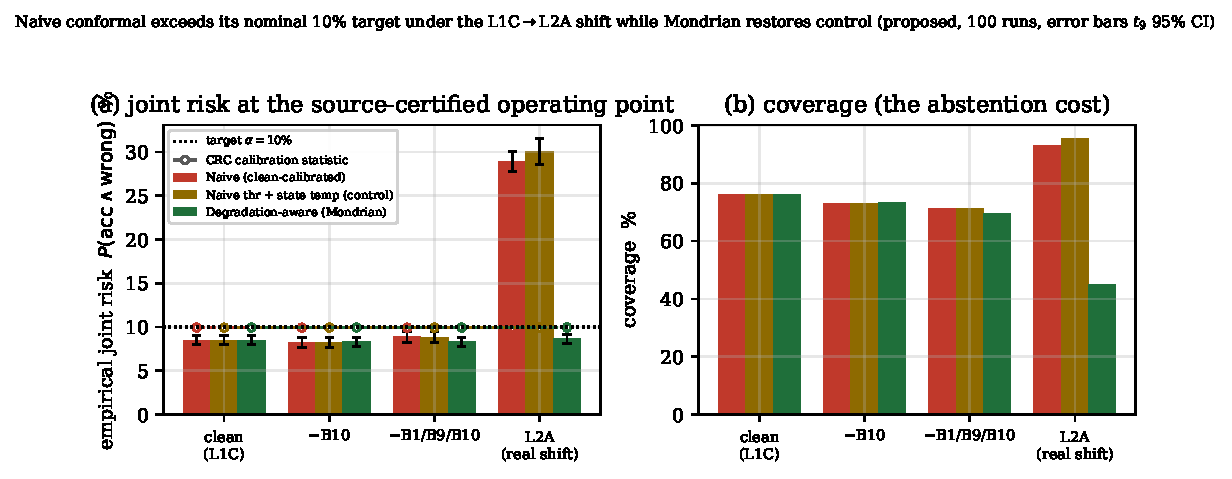
\includegraphics[width=\linewidth]{fig2_flagship_reliability.pdf}
\caption{Naive conformal exceeds its nominal $10\,\%$ target under the L1C$\to$L2A shift while Mondrian restores control (proposed model, 100 runs, two-way cluster-robust SE). (a) empirical joint risk at the certified operating point, per state, with error bars the small-cluster $t_9$ $95\,\%$ CI; (b) coverage, the abstention cost of the remedy. The dashed lines are the CRC calibration selection statistic, which stays $\leq \alpha$ throughout even as the naive L2A risk soars to $28.9\,\%$---the sense in which the failure is silent.}
\label{fig:flagship}
\end{figure}

\paragraph{The dominant mechanism is a stale input-normalization contract, and re-normalizing without labels restores the certificate.} Which part of the reflectance transformation is the certificate sensitive to---the per-pixel spectral distortion of the atmospheric physics, or the shift in each band's radiometric scale? The model normalizes every input with the per-band mean and variance of its \emph{source} (L1C) training data and reuses those statistics on L2A: a stale normalization contract that leaves the atmospherically-rescaled L2A input off the scale the certificate was calibrated on. We test the scale hypothesis directly by re-normalizing the L2A input with its \emph{own} per-band statistics---estimated from the unlabelled deployment product, with no target labels and no change to the trained model, threshold or temperature---before the identical clean-calibrated certificate (five model seeds $\times$ ten calibration splits on the flagship model). Product-aware re-normalization restores the naive joint risk from $28.6 \pm 0.7\,\%$ (reproducing the flagship breach) to $10.2 \pm 0.3\,\%$ at $74\,\%$ coverage, against clean's $8.6\,\%$ at $76\,\%$: an almost complete, \emph{label-free} repair at clean-like coverage, whose small residual above clean is the genuine spectral distortion that a global per-band rescaling cannot undo. The repair is not a transductive artefact of normalizing the evaluation pixels by their own statistics---estimating the statistics on a disjoint calibration split and applying them to the evaluation gives $10.5 \pm 0.2\,\%$, indistinguishable from the pooled $10.2\,\%$. Two consequences reframe the mechanism and remedy that follow. First, the breach is \emph{dominated} by the calibration-to-deployment input-normalization mismatch---a stale contract between the certificate and the model's front end---rather than by the atmospheric physics as such. This does not contradict the failure of weighted conformal above; it explains it. Weighted conformal reweights the calibration distribution while leaving the shifted, miscalibrated confidence scores untouched, so it cannot repair a moved confidence-to-error relationship; product-aware re-normalization instead repairs the model's input \emph{upstream} of the scores, so the relationship the shift had moved is restored at its source rather than reweighted after the fact. Product-aware (test-time) input normalization is itself a long-known covariate-shift remedy \citep{adabn2016,schneider2020,nado2020,benz2021}, and the standard remote-sensing practice of a \emph{fixed} training normalization \citep{corley2024} is exactly the failing naive baseline here. Second, because a re-normalization estimated from unlabelled deployment data restores control at clean-like coverage, the per-stratum (Mondrian) recalibration we study is \emph{one} valid remedy but not the necessary, label-requiring one that the labelled arm alone would suggest: for the atmospheric shift the certificate can be repaired without any target labels or abstention.

\paragraph{A second, algorithmically different atmospheric processor breaks it too.} If the breach were an artefact of Sen2Cor's particular radiometric conventions, a different processor should not reproduce it. We re-ran the flagship with ACOLITE---a dark-spectrum atmospheric correction at a fixed climatological aerosol optical thickness, algorithmically different from Sen2Cor---as an alternative L1C$\to$surface-reflectance product, on the $590$ test patches ACOLITE processed successfully ($181$ of the $184$ scene-components), evaluating every state on that same set with reflectance clipped to a physical range so that a small fraction of over-corrected bright pixels cannot drive the result (ACOLITE additionally omits the B9 water-vapour band, whose removal Table~\ref{tab:banddrop} shows is negligible). The naive certificate breaks to a statistically equivalent degree under the two processors: ACOLITE-surface naive joint risk is $28.6 \pm 0.9\,\%$ (its $t_9$ interval $[26.6, 30.6]$ excluding the target), against $28.6 \pm 0.7\,\%$ for Sen2Cor-L2A on the same patches ($28.56$ and $28.64\,\%$)---their paired per-run difference is $-0.08\,\%$ with a bootstrap interval $[-1.33, +1.16]$ lying within a $\pm 2\,\%$ equivalence margin (a two-one-sided test), so the two independently-implemented corrections break the certificate equivalently rather than merely landing close in point estimate---and $9.3\,\%$ on clean L1C, with Mondrian restoring both ($8.6$ and $8.8\,\%$). That two algorithmically different processors break the source-calibrated certificate near-identically shows the failure is not an artefact of one processor's radiometric conventions; because both implement a broadly similar top-of-atmosphere-to-surface transformation, this points to the L1C$\to$surface-reflectance shift rather than to Sen2Cor specifically, though it does not on its own isolate the atmospheric physics from conventions the two processors may share. Two controls (Appendix~\ref{app:repro}) confirm the comparison is neither an artefact of \emph{which} scenes ACOLITE could process nor of the reflectance clip: the $590$ retained patches match the $385$ ACOLITE-failed ones in cloud cover ($p=0.46$) and latitude ($p=0.36$), and the ACOLITE breach stays within $28.6$--$31.6\,\%$ across no clip, the $[-0.1,1.6]$ clip and a tight $[0,1]$ clip---if anything the clip \emph{lowers} it.

\paragraph{The breach replicates on an independent scene set.} A single test split cannot show the phenomenon is not specific to those $195$ scenes. We therefore repeat the flagship protocol on the official CloudSEN12 \emph{validation} split---$535$ high-quality-labelled patches from $107$ annotation ROIs ($104$ scene-connected components). This split is a random draw from the non-test scenes rather than a spatially blocked hold-out, so while it is disjoint from the test scenes by construction it can share Sentinel-2 products with train; we therefore audited it, found two products also present in train, and dropped their pixels ($0.4\,\%$ of the set) so the replication is genuinely calibration-disjoint from training. We use this split only as an independent replication set, never for model selection or tuning. Training the identical model on the same train split and calibrating and evaluating the CRC on the audited held-out scenes, the failure reproduces: the naive joint risk rises from $8.1\,\%$ on clean L1C to $29.1 \pm 0.8\,\%$ under the L1C$\to$L2A shift (its $t_9$ interval $[27.2, 31.0]$ excluding the target), the confidence ranking degrades in step (AURC $6.2 \to 21.6$, a $3.5\times$ rise), and Mondrian restores the target ($7.1\,\%$) at the same coverage cost ($93 \to 42\,\%$). The per-class collapse recurs as well: mean IoU falls $54.5 \to 28.4$ and the two minority cloud classes collapse almost completely (thin cloud IoU $34.5 \to 1.1$, shadow $35.2 \to 0.9$), their accepted-pixel selective risk reaching $99.9\,\%$, so the confidently-wrong mass concentrates in the same minority classes as on the test split (Table~\ref{tab:classwise}). The magnitude on an entirely separate set of scenes is within a point of the test-split headline, so the atmospheric-certificate failure is a property of the task and shift, not of the particular scenes calibrated on.

\paragraph{Pixel accuracy hides a per-class collapse.} The aggregate accuracy drop understates the operational damage and conceals \emph{which} pixels fail. Decomposing the flagship by class (Table~\ref{tab:classwise}; the full 100-run design), the shift crashes the mean IoU from $54.0$ to $29.3$ and macro-F1 from $67.8$ to $37.4$: the two minority cloud classes---thin cloud and cloud shadow, operationally the hardest and most label-ambiguous \citep{aybar2022cloudsen12}---collapse almost completely (IoU $30.3\to0.4$ and $38.2\to1.4$). That is exactly where the confidently-wrong mass concentrates: at the clean-calibrated operating point, the accepted-pixel error rate (selective risk) on L2A reaches $100\,\%$ for thin cloud and $99.6\,\%$ for cloud shadow, while the dominant clear class retains a low empirical selective risk ($0.3\,\%$). The $28.9\,\%$ overall joint risk is thus not diffuse---it is driven by minority-class failures that overall pixel accuracy masks (the pixel-support-weighted sum of the class-conditional joint risks, $\sum_k w_k R_k$ with $w_k$ the class-$k$ pixel fraction, recovers the $28.9\,\%$ headline), which is why we read the accuracy drop as an \emph{under}-statement of the operational damage. Operationally the confidently-wrong mass is thin cloud and shadow admitted as clear, so any downstream product that trusts the naive certificate---a cloud-screened composite, a surface-reflectance time series---would ingest cloud- and shadow-contaminated pixels precisely where the certificate reports itself in control.

\begin{table}[t]
\centering
\caption{Per-class decomposition of the flagship (proposed model, 100 runs $=10$ splits $\times\,10$ seeds; IoU and the CRC risks are mean $\pm$ two-way cluster-robust SE, coverage is the mean). Pixel accuracy hides the shift's effect: under L2A the minority cloud classes collapse in IoU and the confidently-wrong mass concentrates in them (their accepted-pixel selective risk approaches $100\,\%$), while the dominant clear class retains low selective risk. The per-class quantities are empirical class-conditional risks---conditioned on the true-class pixels---not class-conditional conformal guarantees; the CRC operating-point risks are at the clean-calibrated threshold. Class pixel supports on L2A are clear $51\,\%$, thick cloud $30\,\%$, thin cloud $10\,\%$, cloud shadow $10\,\%$, so the two collapsing minority classes are only ${\sim}19\,\%$ of pixels yet drive the joint risk. All values in \%.}
\label{tab:classwise}
\begin{tabular}{llcccc}
\toprule
state & class & IoU & selective risk & joint risk & coverage \\
\midrule
clean & clear        & $76.4\pm0.2$ & $2.7\pm0.2$ & $2.3\pm0.1$ & 84.6 \\
      & thick cloud  & $71.1\pm0.3$ & $9.2\pm0.4$ & $7.1\pm0.3$ & 76.7 \\
      & thin cloud   & $30.3\pm0.8$ & $58.8\pm2.0$ & $27.3\pm1.1$ & 46.5 \\
      & cloud shadow & $38.2\pm0.8$ & $46.9\pm1.4$ & $27.6\pm1.0$ & 58.7 \\
\midrule
L2A   & clear        & $61.8\pm0.6$ & $0.3\pm0.1$ & $0.3\pm0.1$ & 97.6 \\
      & thick cloud  & $53.5\pm1.6$ & $42.8\pm2.2$ & $37.7\pm1.9$ & 88.1 \\
      & thin cloud   & $\mathbf{0.4\pm0.1}$ & $\mathbf{100.0}$ & $91.5\pm0.8$ & 91.5 \\
      & cloud shadow & $\mathbf{1.4\pm0.4}$ & $\mathbf{99.6}$ & $92.6\pm1.4$ & 92.9 \\
\bottomrule
\end{tabular}
\end{table}

\paragraph{The breach is not an artefact of the weighting.} The certified triple is component-equal-weighted (Section~\ref{sec:unit}) whereas the segmentation accuracy is pixel-level, so we re-evaluated every flagship quantity at the same operating point under the pixel-pooled (sample-weighted) alternative, on an independent $100$-run draw. The two weightings agree to within noise: the L2A naive joint risk is $29.0\,\%$ component-equal versus $29.0\,\%$ pixel-pooled (coverage $93.8$ versus $93.7\,\%$; selective risk $31.0$ versus $31.0\,\%$), and the component-equal accuracy equals the pixel accuracy ($67.3\,\%$). The scene-connected components are close enough in size that the choice of weighting does not move the headline, and the component-equal joint of $29.0 \pm 0.7\,\%$ reproduces the flagship's $28.9\,\%$ on this fresh set of seeds.

\subsection{Two pure deployment shifts: a surface gap that rises above target, a geographic gap that does not}
\label{sec:deployment}
To test whether the failure is specific to the atmospheric shift we construct two further shifts of a different \emph{type} on the same task, holding the input product fixed (clean L1C) so that the shift is \emph{where the model is deployed}, not \emph{what bands it sees}. In each, the naive arm calibrates on held-out source units and is evaluated on unseen target units; the Mondrian arm recalibrates on the target (Fig.~\ref{fig:gaps}). The surface strata (dark: vegetation, cropland, water; bright: built-up, bare soil, snow/ice) and the hemispheric split (by scene-centroid latitude) follow fixed rules; the exact assignment and the per-stratum scene, season and class-proportion breakdown are given in the released code.

\emph{Surface domain gap.} Training and naive-calibrating only on dark surfaces (vegetation, cropland, water) and deploying on the bright surfaces (built-up, bare soil, snow/ice) the model has never seen---the operational cloud-confusion case---raises the naive joint risk above target to $11.35 \pm 0.34\,\%$, its small-cluster $t_9$ interval $[10.6, 12.1]$ excluding $10\,\%$, although a scene-component bootstrap over the $33$ bright units is less conclusive ($[9.3, 13.6]$, Section~\ref{sec:method}); Mondrian restores it to $2.42 \pm 0.21\,\%$. The plain-MLP-with-band-group-dropout baseline (b2) mirrors this ($11.9 \to 2.5\,\%$), so the effect is not architecture-specific.

\emph{Geographic domain gap.} Training and calibrating on the Northern hemisphere and deploying on the unseen Southern hemisphere, under the identical 100-run design, shows no clear evidence of exceeding the target: the proposed model's naive joint risk on Southern units is $9.79 \pm 0.23\,\%$ (its $t_9$ interval $[9.3, 10.3]$ and a scene-component bootstrap $[9.1, 12.4]$ both including the $10\,\%$ target), and the plain-MLP baseline likewise straddles it ($10.12 \pm 0.23\,\%$, $t_9$ interval $[9.6, 10.6]$). Neither is the clear violation the surface gap produced. Accuracy also transfers well ($79\,\%$ on Southern units), consistent with Northern and Southern mid-latitudes sharing surface and cloud regimes. Mondrian still lowers the risk further (proposed $5.8\,\%$), but from an already-controlled starting point.

The surface and geographic axes are both pure deployment shifts on a fixed input, so the contrast is between two operational shifts of different kinds; we do not claim they differ only along a single measured gap dimension---the surface and hemisphere splits also differ in class prevalence, season and biome. The structural surface gap (dark training surfaces to spectrally very different bright ones) breaks the naive certificate; the milder geographic gap (regions that share surface and cloud regimes) does not. A direct paired bootstrap of the surface-minus-geographic difference confirms this is more than a one-significant-one-not artefact: the difference is $+1.56\,\%$, its $95\,\%$ interval $[+1.11, +2.02]$ excluding zero, so the surface axis breaches significantly more than the geographic one---though both sit close to the target in absolute terms. This is an illustrative contrast between two deployment shifts: the surface gap raises the risk above target, while the milder geographic gap gives no clear evidence of a breach. We read it as suggestive of a \emph{conditional} failure---one that appears under the bright-surface split but not the hemisphere split---rather than as a general diagnosis or a claim that severity tracks a measured gap size. The atmospheric shift breaks harder still ($28.9\,\%$) but also changes the input representation, so we read it as a stronger, different-mechanism confirmation rather than another point on the same deployment-gap scale.

On the surface axis the Mondrian arm recalibrates on a median of only ${\sim}12$ scene-component units (versus ${\sim}91$ for the naive arm and ${\sim}69$ for the flagship). At $\alpha = 10\,\%$ this is near the conformal feasibility floor, so the restored $2.4\,\%$ at $41\,\%$ coverage (full triple in Table~\ref{tab:deploytriple}) reflects heavy, conservative over-abstention on a small target stratum rather than a tight guarantee at target---we report it as restoring \emph{control at a large coverage cost}.

\begin{figure}[t]
\centering
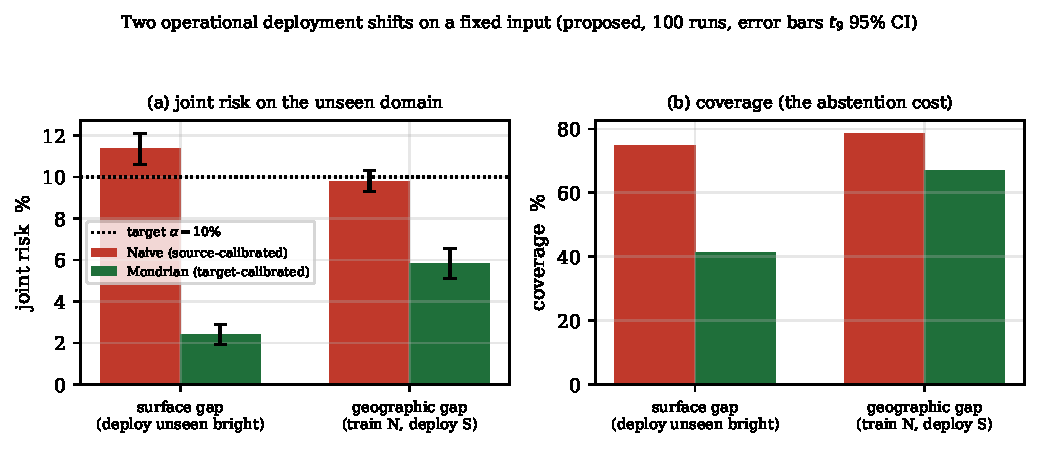
\includegraphics[width=0.6\linewidth]{fig3_domain_gaps.pdf}
\caption{Naive versus Mondrian joint risk on the unseen target domain, for the surface and geographic deployment shifts (proposed model). The structural surface gap raises the risk above the $10\,\%$ target (scene-sensitively); the milder geographic gap does not.}
\label{fig:gaps}
\end{figure}

\begin{table}[t]
\centering
\caption{Full operating-point triple for the two deployment shifts (proposed model, 100 runs; joint-risk SE two-way cluster-robust). Reporting selective risk and coverage alongside the joint risk shows that the surface Mondrian's low joint risk ($2.4\,\%$) is bought with heavy abstention (coverage $41\,\%$) rather than a genuinely reliable accepted set, and that the geographic naive arm is already near target. Accuracy is on the target domain. All values in \%.}
\label{tab:deploytriple}
\begin{tabular}{llcccc}
\toprule
shift & arm & joint risk & selective & coverage & accuracy \\
\midrule
surface    & naive    & $11.35\pm0.34$ & $15.2\pm0.5$ & $74.7\pm1.0$ & $75.3\pm0.8$ \\
           & Mondrian & $2.42\pm0.21$  & $5.8\pm0.3$  & $41.2\pm2.1$ & $75.3\pm0.8$ \\
\midrule
geographic & naive    & $9.79\pm0.23$  & $12.5\pm0.4$ & $78.7\pm0.7$ & $79.2\pm0.6$ \\
           & Mondrian & $5.83\pm0.33$  & $8.7\pm0.5$  & $67.1\pm0.7$ & $79.2\pm0.6$ \\
\bottomrule
\end{tabular}
\end{table}

\subsection{Model-class dependence}
\label{sec:modelclass}
We run a frozen channel-adaptive foundation model \citep[DOFA,][]{xiong2024dofa} through the \emph{identical} flagship protocol---the same CRC joint-risk estimand, the scene-connected-component unit, the $10 \times 10$ crossed design, and the two-way cluster-robust SE---so the CRC \emph{protocol} is identical across the two models, though their capacity, pretraining and spatial context are not. DOFA is \emph{far more} reliable than the small per-pixel model under the L1C$\to$L2A shift: naive joint risk $9.95 \pm 0.21\,\%$ versus $28.9\,\%$ for the small model. Its L2A joint risk sits right at the $10\,\%$ target (its small-cluster $t_9$ interval $[9.5, 10.4]$ including it), so a clear residual breach cannot be established; Mondrian lowers it to $8.78 \pm 0.19\,\%$, and the abstention cost is far gentler than the flagship's (coverage $79.7 \to 76.4\,\%$, versus $93 \to 45\,\%$ for the small model). DOFA is not immune, however: under a spectral-band-drop shift (removing its two SWIR bands) its naive joint risk rises to $11.69 \pm 0.37\,\%$, its $t_9$ interval $[11.0, 12.4]$ excluding the target---a breach now certified over the full $10 \times 10$ design---and Mondrian brings it to $8.66 \pm 0.36\,\%$. The reliability crisis is thus \emph{model-dependent} in this two-model comparison: a channel-adaptive foundation model largely escapes it under the atmospheric shift but shows a modest, certified breach under a band-drop shift, and we do not claim a universal failure. We cannot fully decompose \emph{which} of DOFA's differences produces the greater reliability, but first principles narrow them. Channel-adaptivity is not the differentiator: our small model is itself a wavelength-conditioned band-as-modality encoder. Two differences are mechanistically pointed. First, DOFA's fixed nine-band input omits the water-vapour band B9, whose reflectance shifts most of any band under the L1C$\to$L2A correction (by ${\sim}{+}0.2$--$0.3$ here), while the flagship's thirteen-band input uses it: a model that never sees the most atmospherically-volatile band is by construction less exposed to the shift, so a fully fair model-class comparison would additionally control the band set. We test this directly: a plain per-pixel MLP---no spatial context, no pretraining---trained and calibrated identically on three band sets breaks the naive certificate to $48.4 \pm 0.2\,\%$ on all thirteen L1C bands, but to only $29.2 \pm 0.5\,\%$ once B9 alone is removed and $23.8 \pm 0.3\,\%$ on DOFA's exact nine bands. Dropping the single most volatile band thus accounts for most of the band-set effect, and the band set as a whole roughly halves the breach---a concrete, quantified contributor to DOFA's greater reliability that a fair comparison must control. It does not close the gap on its own, though: even the nine-band per-pixel MLP ($23.8\,\%$) sits far above DOFA's $9.9\,\%$, leaving the residual to DOFA's spatial context and pretraining. Second, DOFA's spatial context can resolve the per-pixel-ambiguous thin-cloud and shadow pixels that drive the breach from their spatial neighbourhood, which a per-pixel model cannot; its cross-modal pretraining plausibly adds shift-stable features on top. These causes are entangled and we claim no decomposition: the escape is multi-causal, with the band set a concrete contributor a fair comparison must control, so we read the DOFA result as establishing that a different model \emph{class} largely escapes the failure, not the single mechanism behind it. (This is a foundation-model \emph{feature} baseline---a frozen encoder with a light trainable head, not the official DOFA segmentation recipe.) DOFA's Sentinel-2 pretraining imagery derives from SatlasPretrain \citep{bastani2023}, which samples the global 2016--2022 archive; because CloudSEN12's 2018--2020 acquisitions fall inside that envelope, incidental scene overlap cannot be fully excluded. But DOFA is pretrained self-supervised on raw reflectance with no cloud labels and is used here only as a frozen extractor (no fine-tuning), and SatlasPretrain preferentially retains low-cloud scenes whereas CloudSEN12 targets cloudy ones, so any overlap is non-systematic and introduces no cloud-mask label information into our result, though we cannot exclude that pretraining exposure shapes its representation.

\paragraph{Spatial context, isolated in one harness, attenuates the breach without removing it, and the label-free fix generalizes.} DOFA differs from the per-pixel model in band set, spatial context and pretraining at once. We isolate the \emph{spatial-context} contribution within a single harness: on DOFA's exact nine bands, trained from scratch with no pretraining, we compare a per-pixel MLP against a spatial U-Net through the identical certificate, evaluating both on the same sampled pixels of the same scene-components (five model seeds $\times$ ten calibration splits, BatchNorm- and depth-matched so that spatial context is the only structural difference). Both breach under the stale L1C normalization---the per-pixel MLP to $24.2 \pm 0.6\,\%$ (reproducing the $23.8\,\%$ nine-band control above) and the spatial U-Net to $13.1 \pm 0.7\,\%$, its small-cluster $t_4$ interval $[11.3, 15.0]$ excluding the target---so the failure is \emph{not} a per-pixel artefact: a representative spatial segmentation model, which also attains higher clean accuracy ($82\,\%$ versus $77\,\%$), breaks the certificate too. But spatial context attenuates the severity by $11$ points within this one harness ($24.2 \to 13.1\,\%$), and adding pretraining takes DOFA the rest of the way to $9.9\,\%$. The gradient is coherent---per-pixel $24.2\,\%$, spatial-from-scratch $13.1\,\%$, spatial-and-pretrained $9.9\,\%$---so the reliability crisis is model-\emph{class}-dependent: most severe for the per-pixel spectral model and progressively attenuated by spatial context and then pretraining, neither universal nor a per-pixel artefact. The label-free remedy generalizes with the failure: product-aware re-normalization restores \emph{both} models to the target at clean-like coverage (per-pixel $24.2 \to 8.7\,\%$ at $69\,\%$ coverage, U-Net $13.1 \to 8.9\,\%$ at $83\,\%$), so the input-normalization contract diagnosed on the flagship is not specific to its architecture.

\begin{table}[t]
\centering
\small
\caption{The naive certificate's confidently-wrong (joint) risk and its per-stratum (Mondrian) restoration across every condition tested, against the $10\,\%$ target (mean $\pm$ two-way cluster-robust SE, \%). The atmospheric breach reproduces under a second, algorithmically different processor, on held-out validation scenes, and---separately---across target risks $5$--$20\,\%$, and a covariate-shift weighted-conformal threshold---a likelihood-ratio approximation or confidence-density heuristic---does not repair it ($32.7\,\%$), whereas a label-free product-aware re-normalization restores it to $10.2\,\%$ at $74\,\%$ coverage. Among pure deployment shifts it is conditional; under the identical protocol a channel-adaptive foundation model is far more reliable to the atmospheric shift, and a one-harness spatial-context isolation (per-pixel MLP $24.2\,\%$, spatial U-Net $13.1\,\%$ on nine bands) attributes part of that gap to spatial context. Breach $=$ the small-cluster $t$ interval excludes the target.}
\label{tab:summary}
\begin{tabular}{lccl}
\toprule
Condition & Naive & Mondrian & Verdict \\
\midrule
\multicolumn{4}{@{}l}{\emph{Atmospheric shift L1C$\to$L2A, small per-pixel model}} \\
\quad Sen2Cor, test (flagship)    & $28.9 \pm 0.5$ & $8.6$ & breach \\
\quad ACOLITE, test               & $28.6 \pm 0.9$ & $8.8$ & breach \\
\quad Sen2Cor, validation scenes  & $29.1 \pm 0.8$ & $7.1$ & breach \\
\midrule
\multicolumn{4}{@{}l}{\emph{Deployment shift (input fixed), small per-pixel model}} \\
\quad Surface, dark$\to$bright    & $11.4 \pm 0.3$ & $2.4$ & breach$^{\dagger}$ \\
\quad Geographic, North$\to$South & $9.8 \pm 0.2$  & $5.8$ & no breach \\
\midrule
\multicolumn{4}{@{}l}{\emph{Foundation model (DOFA), identical protocol}} \\
\quad Atmospheric L1C$\to$L2A     & $9.9 \pm 0.2$  & $8.8$ & no clear breach \\
\quad Spectral band drop (SWIR)   & $11.7 \pm 0.4$ & $8.7$ & breach \\
\bottomrule
\end{tabular}

\vspace{2pt}
{\footnotesize $^{\dagger}$ scene-composition-sensitive: significant under the two-way SE, but its scene-component bootstrap dips below the target.}
\end{table}

\section{Discussion and limitations}
\label{sec:disc}
We lead with the limitations, because several bound the claims directly.

\paragraph{Coverage and selective risk are part of the result, not a footnote.} The certified quantity is a joint mass, which any method drives to zero by abstaining. Mondrian's restoration is therefore genuine but partial: on the flagship it accepts $45\,\%$ of pixels where naive accepts $93\,\%$, and even among those it accepts the error rate is $19.4\,\%$, not $\leq\!10\,\%$---what is controlled is the \emph{joint} confidently-wrong mass, not the accepted-pixel error rate. The operational reading is that per-stratum recalibration converts a silent, uncontrolled joint error mass into an \emph{explicit} accuracy--coverage trade the operator can see and choose. We report every risk with both its coverage and its selective error precisely so this trade is never hidden.

\paragraph{Whether the crisis occurs is conditional.} The surface and geographic axes are both pure deployment shifts on a fixed input, so the comparison is between two deployment shifts of different kinds: the structural surface gap raises the risk above target ($11.4\,\%$, its small-cluster $t_9$ interval excluding the target), while the milder geographic gap shows no clear evidence of a breach ($9.8\,\%$, its $t_9$ interval including the target). The failure appears under a structural domain gap between calibration and deployment but not under the milder geographic split---conditional on the kind of shift, not a consequence of mere geographic distance. The atmospheric shift breaks harder ($28.9\,\%$) but also changes the input representation, so we read it as a stronger, different-mechanism confirmation. We do not claim a smooth monotone ``severity $= f(\text{gap size})$'' law---an independently-measured gap metric across more shift types would be needed---and we read the surface-above-target / geography-shows-no-clear-breach pair as an illustrative contrast of two deployment shifts, not a general diagnosis. The crisis is also model-dependent---a larger pretrained foundation model is far more reliable under the atmospheric shift, so the severity does depend on the model, with the small per-pixel model suffering it most---though our single same-protocol comparison cannot isolate which of the foundation model's differences (capacity, pretraining, channel-adaptivity, spatial context) is responsible.

\paragraph{Scope of the evidence.} The magnitude is measured on one benchmark (CloudSEN12); its test metadata records eight distinct Sen2Cor product-baseline versions, a mild internal heterogeneity we do not control for. We have, however, stressed the finding along every axis this benchmark affords: two algorithmically different atmospheric processors (Sen2Cor and ACOLITE) break it to a statistically equivalent degree, it replicates on the official held-out validation scenes (audited for shared train products, $29.1\,\%$ versus the $28.9\,\%$ headline), it survives target risks from $5$ to $20\,\%$ and both deployment-shift axes, and it is model-class-dependent (a channel-adaptive foundation model largely escapes it). What remains outside this benchmark's reach is a \emph{fully independent} cloud dataset with its own labelling protocol and geography; because no public Sentinel-2 cloud-segmentation dataset ships paired L1C/L2A at CloudSEN12's expert label quality, establishing the magnitude on a second dataset requires re-processing raw products through an atmospheric-correction pipeline and is the most direct further strengthening.

\paragraph{The mechanism is borrowed; the comparison is not compute-matched.} Our band-as-modality architecture is a substrate of cited components, and the proposed-vs-MLP comparison is not matched on training compute, optimiser steps, or data exposure. The paper's claim is the \emph{within-method} naive-vs-Mondrian gap, invariant to that confound because both arms share the trained model; the plain-MLP baseline reproducing the surface-axis result ($11.9 \to 2.5\,\%$) shows the finding does not depend on it.

\paragraph{Statistical caveats.} The exchangeable unit is the scene-connected component and the standard error is two-way cluster-robust; these were found by adversarial review and change the confidence intervals, not the direction of the result. The scene-connected component is a reasonable operational approximation to exchangeability, not a proof of it: residual dependencies remain---the same annotation region on different dates, adjacent regions, a shared acquisition or atmospheric system, and the reuse of a component across the Monte-Carlo splits. The seed-cluster bootstrap, seed-only aggregation and a scene-component bootstrap of the evaluation composition (Section~\ref{sec:method}) leave the flagship breach intact; for the borderline surface breach we additionally ran a nested scene-component bootstrap that re-runs the entire calibration pipeline on each of $1500$ resamples---re-drawing source and target components, re-splitting temperature and calibration, re-fitting the temperature and re-selecting the CRC threshold---so that it propagates calibration-composition uncertainty most fully. Its $95\,\%$ interval is $[9.6, 14.7]$ (mean $12.1\,\%$): the point estimate remains above target but the interval now includes $10\,\%$, so under full calibration resampling the surface breach is inferentially inconclusive---consistent with the evaluation-only bootstrap ($[9.3, 13.6]$) and reinforcing our reading of it as suggestive rather than settled. With only 10 clusters on each factor our cluster-robust intervals are themselves small-cluster approximations; we therefore read the borderline geographic axis as suggestive rather than settled. \citet{barber2023}'s coverage-gap bound is worst-case and does not predict our exact numbers. The estimand is the mean risk on a fixed per-patch pixel sample (one sampling seed across runs), so our standard error reflects the calibration-split and model-seed variation, not pixel-sampling variability---a residual source we bound by using several hundred pixels per patch but do not fully propagate.

\paragraph{Implications.} For operational Earth observation the practical message is narrow and actionable: a model must not be assumed \emph{reliable} under a shift on the strength of its \emph{aggregate} accuracy---which can hold up while hiding a per-class collapse and a silent certificate failure---and a conformal or selective-prediction operating point calibrated before deployment should be treated as valid only within the calibration regime. The failure we characterise is the \emph{silent} reuse of one certificate when the shift is not flagged as a distinct operational state: an unlabelled processing-baseline change, a gradual sensor drift, or a pipeline that freezes its input normalization and threshold at training time. The remedies form a hierarchy of increasing cost. When the shift is a known input-processing change that the scene metadata already records---the L1C-versus-L2A product level is the clearest case---the first response needs \emph{no labels}: re-normalize each product with its own statistics before inference, which on the atmospheric shift restores the certificate at clean-like coverage (Section~\ref{sec:flagship}). The operational contract is simply that the input normalization travel with the product rather than be frozen at training time; a metadata gate on product level triggers it automatically. Where a residual remains, or the operational state is discrete but not a mere normalization change (our surface gap), per-stratum (Mondrian) recalibration is the next safeguard, at a cost the operator can see and choose---target-state labels to recalibrate on, and abstention. Where the shift is continuous or unknown, the weighted- and adaptive-conformal machinery we deliberately did not invoke is the natural next tool, and quantifying its cost under the same operational shifts is future work.

\paragraph{Companion analyses, not load-bearing.} Two further analyses inform but do not carry the main result, so we summarise them here rather than as main experiments. A training-ingredient decomposition (band-group dropout versus channel-sampling regularisers \citep{bao2024channelvit,pham2024dichavit}, released with the code) identifies which mechanism supplies the missing-band robustness the reliability study presupposes, and---more to the point---shows that robustness measured under \emph{synthetic} band removal overstates it under \emph{physically-grounded} (6S) band loss, reinforcing our choice to measure reliability under a real rather than a simulated shift. An exploratory external anchor---EMIT's physics-based per-band retrieval uncertainty \citep{green2020emit,thompson2018isofit} over $N=14$ granules---aligns only weakly and inconsistently with our per-band reconstruction anomaly (per-pixel correlation $+0.04$), so we treat it as suggestive at most. The load-bearing evidence remains the CloudSEN12 conformal experiments.

\section{Conclusion}
Robustness certification is not reliability certification. On real Sentinel-2 cloud segmentation, under the operational L1C$\to$L2A atmospheric-correction shift a model's \emph{aggregate} accuracy understates the operational damage (a 12-point drop that masks a per-class collapse) while a naive conformal certificate comes to admit more than three times the confidently-wrong risk it reports---silently, because the statistic the certificate minimises still passes. The failure is not confined to that one shift, nor is it universal: two pure deployment shifts illustrate the condition---a structural surface gap raises the risk above target, while a milder geographic gap shows no clear evidence of a breach---so whether the crisis occurs is conditional on the kind of shift, not on shift alone. The severity is also model-dependent: spatial context and then pretraining progressively attenuate it, from the per-pixel spectral model through a from-scratch spatial U-Net to a pretrained foundation model. The atmospheric breach is, at root, a stale input-normalization contract---re-normalizing each product with its own unlabelled statistics restores the certificate without target labels---while per-stratum recalibration restores control more generally, at an abstention cost we report rather than hide; and a defensible certificate on this data requires a scene-connected-component exchangeable unit and a cluster-robust variance that naive alternatives get wrong. We contribute what is, to our knowledge, the first measurement of the robustness $\neq$ reliability decoupling for a conformal certificate under a real atmospheric-correction shift on Sentinel-2, together with an initial characterisation of when it occurs, its trace to a stale product-normalization contract, and a label-free re-normalization that repairs it---a small, honest, and we hope useful correction to how spectral segmentation models are trusted in deployment.

\section*{Data and code availability}
Code, committed result tables, the conformal risk-control implementation, and the Sentinel-2-product-to-scene-component mapping (the test products, their 184 scene-connected components, and the products that span two annotation ROIs) are available at \url{https://github.com/thc1006/band-as-modality-hsi} (commit \texttt{eae9962}). CloudSEN12 \citep{aybar2022cloudsen12}, EMIT and ESA WorldCover are public.

\appendix
\section{Reproducibility details}
\label{app:repro}
\emph{Data and exchangeable unit.} We use the manually-annotated \emph{high}-quality tier of CloudSEN12 \citep{aybar2022cloudsen12}, with co-registered L1C (13-band TOA reflectance) and L2A (12-band Sen2Cor BOA reflectance) products for the identical pixels. The $195$ test annotation ROIs form $184$ scene-connected components (ROIs sharing any Sentinel-2 product identifier are unioned; $12$ products span two ROIs, merging $11$ units). Four products appear in both the shipped train and test splits; we drop their test patches before any calibration, leaving the $184$-component structure intact. Each run draws a fixed per-patch pixel sample (one sampling seed) of several hundred pixels per patch.

\emph{Preprocessing and training.} Each band's integer digital number is converted to reflectance by the standard $\times 10^{-4}$ scaling and then per-band standardised (z-scored) with the mean and standard deviation of the \emph{training} (L1C) pixels---the stale normalization contract of Section~\ref{sec:flagship}; the product-aware arm replaces only these two per-band statistics with those of the unlabelled deployment product and changes nothing else. L2A carries $12$ bands (B10 absent), placed at their L1C band indices with B10 zero-filled; nodata-filled and int16-saturated pixels are screened by a reflectance-profile guard. The band-as-modality encoder (grouped-band tokenisation, wavelength-conditioned positional encoding, spectral-group masked-autoencoder pretraining for $25$ epochs, band-group dropout) and the plain-MLP baselines (one hidden layer of width $256$) are trained with Adam (learning rate $10^{-3}$, batch size $256$) under an \emph{unweighted} cross-entropy loss for $40$ supervised epochs; DOFA is used as a frozen encoder with a light trainable head. Exact values are in the released code.

\emph{Design and splits.} The flagship and the two deployment axes use $10$ calibration splits $\times\,10$ model seeds ($100$ runs); the $184$ components split deterministically into $46$ temperature, $69$ calibration and $69$ evaluation units per run. Temperature is fitted on a component-disjoint set from the CRC calibration set.

\emph{Deployment strata.} The surface axis trains and naive-calibrates on ESA WorldCover \citep{zanaga2021worldcover} dark codes (\{10, 20, 30, 40, 80, 90, 100\}) and deploys on bright codes (\{50, 60, 70\}: built, bare, snow/ice), a $152$-dark / $33$-bright split of the test components; the geographic axis trains on the Northern hemisphere and deploys on the Southern (scene-centroid latitude $<0$).

\emph{Variance and intervals.} Standard errors are two-way cluster-robust over the split $\times$ seed design \citep{cameron2011}; intervals use the small-cluster $t_9 = 2.262$ critical value. Sensitivity is checked with a seed-cluster bootstrap, seed-only aggregation, and a scene-component bootstrap ($4000$ resamples of the exchangeable units at the fitted operating point). AURC integrates the component-equal selective risk over coverage; AUGRC integrates the joint (generalized) risk; the failure-detection AUROC is the rank probability that a misclassified pixel (the positive class) scores below a correct one. The risk--coverage curve is evaluated at each distinct confidence value, equal-confidence pixels forming one permutation-invariant tie-block that contributes its selective risk times its coverage increment, with coverage running from zero (accept-nothing); the area is therefore the coverage-weighted mean of the cumulative selective risk---a mean-of-cumulative-risks estimator, not a per-point trapezoid, so a lone confident error yields $\mathrm{AURC}=1$.

\emph{Second processor.} ACOLITE (generic distribution, commit \texttt{d5e4cb0}; LUT ACOLITE-LUT-202110) is run with a fixed climatological aerosol optical thickness (dark-spectrum estimate disabled) so that it is a different implementation from Sen2Cor; $590$ of $975$ test patches processed successfully ($181$ scene-components), and reflectance is clipped to $[-0.1, 1.6]$ across all products (physical surface reflectance is nominally $[0,1]$; the range keeps a small margin for correction noise and legitimate bright-cloud reflectance while removing ACOLITE's dark-spectrum over-corrections---negative values and the int16 saturation near $3.3$) so that the ${\sim}0.7\,\%$ of over-corrected bright pixels does not drive the comparison. Two robustness checks support the comparison. (i)~\emph{Retained-subset representativeness}: the $590$ ACOLITE-processed patches are statistically indistinguishable from the $385$ ACOLITE-failed ones in cloud coverage (Mann--Whitney $p=0.46$), scene latitude ($p=0.36$) and label quality, differing only mildly in land cover and difficulty; and Sen2Cor-L2A evaluated on the retained subset ($28.6\,\%$) already equals the full-test breach ($28.9\,\%$), so the subset is representative of the phenomenon. (ii)~\emph{Clip insensitivity}: the clip touches only $0.7\,\%$ of ACOLITE pixels, and re-running the entire train-and-evaluate pipeline ($3$ model seeds) under no clip, the $[-0.1,1.6]$ clip and an aggressive $[0,1.0]$ clip gives ACOLITE-surface naive joint risks of $31.0$, $28.6$ and $31.6\,\%$ respectively---a $3$-point spread all far above target, with the paper's clip giving the \emph{smallest} breach (so it does not inflate the result) and its $3$-seed value reproducing the $10$-seed headline ($28.56\,\%$).

\emph{Weighted conformal.} The covariate-shift weighted threshold (Section~\ref{sec:flagship}) estimates the likelihood ratio $w(x)=\mathrm{d}P_{\mathrm{L2A}}/\mathrm{d}P_{\mathrm{clean}}(x)$ with an $\ell_2$-regularised logistic domain classifier on the temperature-scaled softmax of the temperature split (clean $=0$, L2A $=1$; disjoint from the calibration and evaluation sets); the weights are the classifier odds clipped to $[10^{-3},10^{3}]$, and the deployed threshold is the smallest confidence whose $w$-weighted calibration joint risk is $\leq\alpha$. The domain classifier separates clean from L2A with AUROC $0.80$, and the effective sample size after weighting is $61\,\%$ of the calibration set; the confidence-density heuristic instead reweights by the ratio of L2A-to-clean confidence densities. A synthetic pure-covariate-shift control (fixed $P(Y\!\mid\!X)$, shifted $P(X)$) confirms the implementation recovers control when its assumption holds (naive $6.6\,\%$, heuristic $7.1\,\%$), so the L2A failure is an assumption-violation, not a defective weighting.

\bibliographystyle{elsarticle-harv}
\bibliography{refs}

\end{document}
